\documentclass{article}
\usepackage{fancyhdr}
\usepackage{ctex}
\usepackage{listings}
\usepackage{graphicx}
\usepackage[a4paper, body={18cm,22cm}]{geometry}
\usepackage{amsmath,amssymb,amstext,enumerate,graphicx}
\usepackage{float,abstract,booktabs,indentfirst,amsmath}
\usepackage{array}
\usepackage{booktabs}
\usepackage{multirow}
\usepackage{url}
\usepackage{diagbox}
\renewcommand\arraystretch{1.4}
\usepackage{indentfirst}
\setlength{\parindent}{2em}
\usepackage{enumerate}
\setmonofont{Consolas}
\usepackage{listings}
\usepackage{xcolor}
\usepackage{makecell}
\usepackage{enumitem}
\usepackage{tikz}
\usepackage{wrapfig}
\usepackage{tkz-euclide}
\usepackage{pgfplots}
\usepackage{multicol}
\setfontfamily{\timesfont}{Times New Roman}

\begin{document}

\newcommand{\titem}[1]{
~\\
\begin{itemize}
    \item \heiti \large {#1}
\end{itemize}
}

\newcommand{\bb}[1]{{\heiti {#1}}}

\renewcommand{\d}{\mathrm{d}}

\newcommand{\cf}[1]{$^{#1}\textrm{C}$}

\title{《数学建模及其MATLAB实现》第六次课程作业}
\author{李鹏达}
    

\begin{center}
    \LARGE \textbf{\heiti 《数学建模及其{\timesfont MATLAB}实现》第六次课程作业} \\[0.5em]
    \large 李鹏达 10225101460
\end{center}

确定下列各方程的平衡点属于什么类型,并用 Matlab 或 Python 绘制相图(相轨线),并确定平衡点的稳定性.

\begin{multicols}{2}
    \noindent
    \textbf{(1)} 
    \[
    \begin{cases}
    \frac{dx}{dt} = -2x \\
    \frac{dy}{dt} = -3y
    \end{cases}
    \]

    \noindent
    \textbf{(2)} 
    \[
    \begin{cases}
    \frac{dx}{dt} = 3x \\
    \frac{dy}{dt} = x + 3y
    \end{cases}
    \]

    \columnbreak

    \noindent
    \textbf{(3)} 
    \[
    \begin{cases}
    \frac{dx}{dt} = y \\
    \frac{dy}{dt} = -x
    \end{cases}
    \]

    \noindent
    \textbf{(4)} 
    \[
    \begin{cases}
    \frac{dx}{dt} = 2x + 3y \\
    \frac{dy}{dt} = x + 3y
    \end{cases}
    \]
\end{multicols}

\noindent\textbf{{\heiti 解答:}}

\begin{enumerate}[label=(\arabic*)]
    \item 
    解$
    \begin{cases}
        -2x = 0 \\
        -3y = 0
    \end{cases}
    $
    得平衡点为$P(0, 0)$.

    系数矩阵 $A = \begin{bmatrix} -2 & 0 \\ 0 & -3 \end{bmatrix}$,
    特征方程为 $|A - \lambda I| = 0$, 即
    $$
    \begin{vmatrix}
        -2 - \lambda & 0 \\
        0 & -3 - \lambda
    \end{vmatrix} = \lambda^2 + 5\lambda + 6 = 0
    $$
    解得特征值 $\lambda_1 = -2, \lambda_2 = -3\quad (p=5, q=6)$.

    这是一个稳定的结点.

    其相图如下所示:

    \begin{figure}[H]
        \centering
        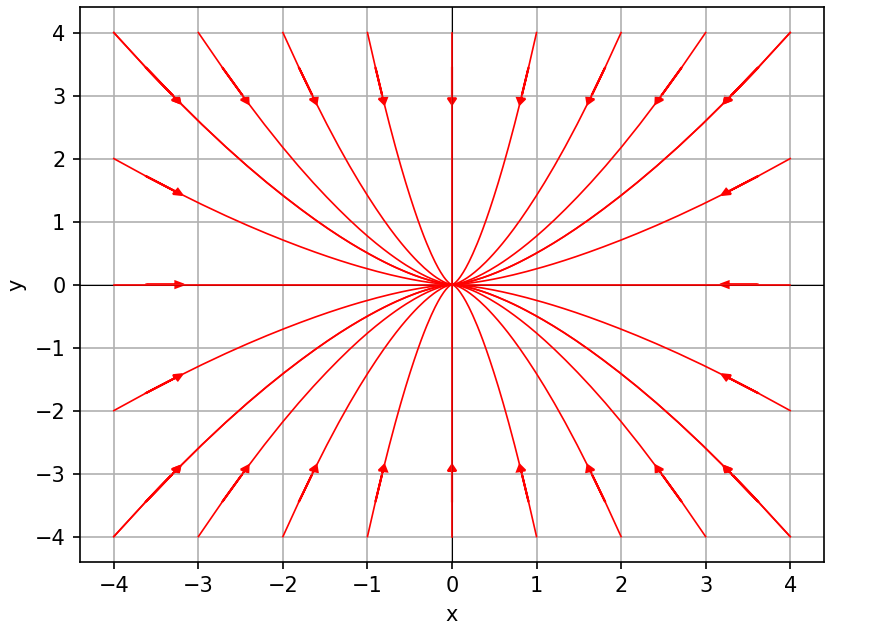
\includegraphics[width=0.4\textwidth]{img/1.png}
        \caption{(1)的相图}
    \end{figure}

    \item
    
    解$
    \begin{cases}
        3x = 0 \\
        x + 3y = 0
    \end{cases}
    $
    得平衡点为$P(0, 0)$.

    系数矩阵 $A = \begin{bmatrix} 3 & 0 \\ 1 & 3 \end{bmatrix}$,
    特征方程为 $|A - \lambda I| = 0$, 即

    $$
    \begin{vmatrix}
        3 - \lambda & 0 \\
        1 & 3 - \lambda
    \end{vmatrix} = \lambda^2 - 6\lambda + 9 = 0
    $$
    解得特征值 $\lambda_1 = \lambda_2 = 3\quad (p=-6, q=9)$.

    这是一个不稳定退化结点.

    其相图如下所示:

    \begin{figure}[H]
        \centering
        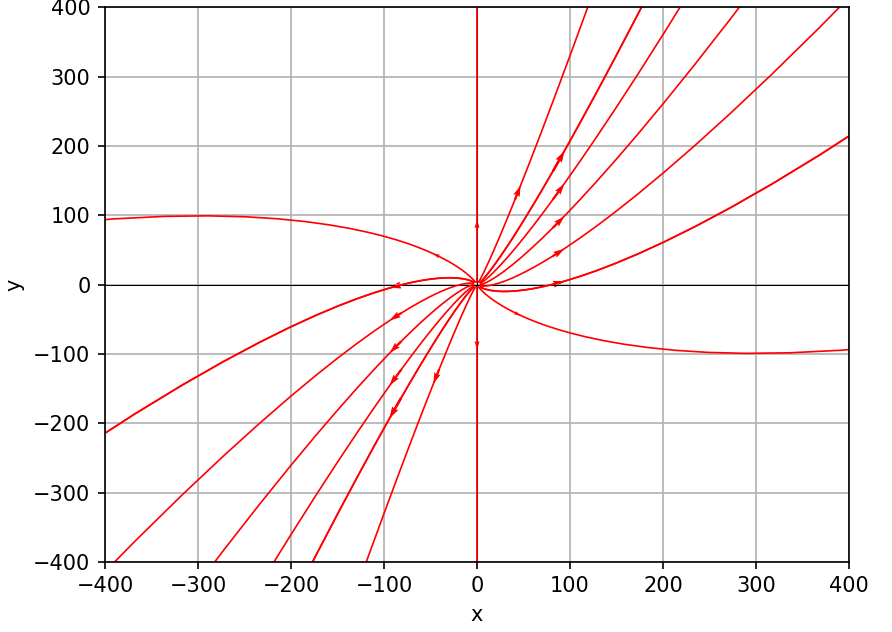
\includegraphics[width=0.4\textwidth]{img/2.png}
        \caption{(2)的相图}
    \end{figure}

    \item 
    
    解$
    \begin{cases}
        y = 0 \\
        -x = 0
    \end{cases}
    $
    得平衡点为$P(0, 0)$.

    系数矩阵 $A = \begin{bmatrix} 0 & 1 \\ -1 & 0 \end{bmatrix}$,
    特征方程为 $|A - \lambda I| = 0$, 即

    $$
    \begin{vmatrix}
        -\lambda & 1 \\
        -1 & -\lambda
    \end{vmatrix} = \lambda^2 + 1 = 0
    $$
    解得特征值 $\lambda_1 = i, \lambda_2 = -i\quad (p=0, q=1)$.

    平衡点类型为中心,稳定性为不稳定.

    其相图如下所示:

    \begin{figure}[H]
        \centering
        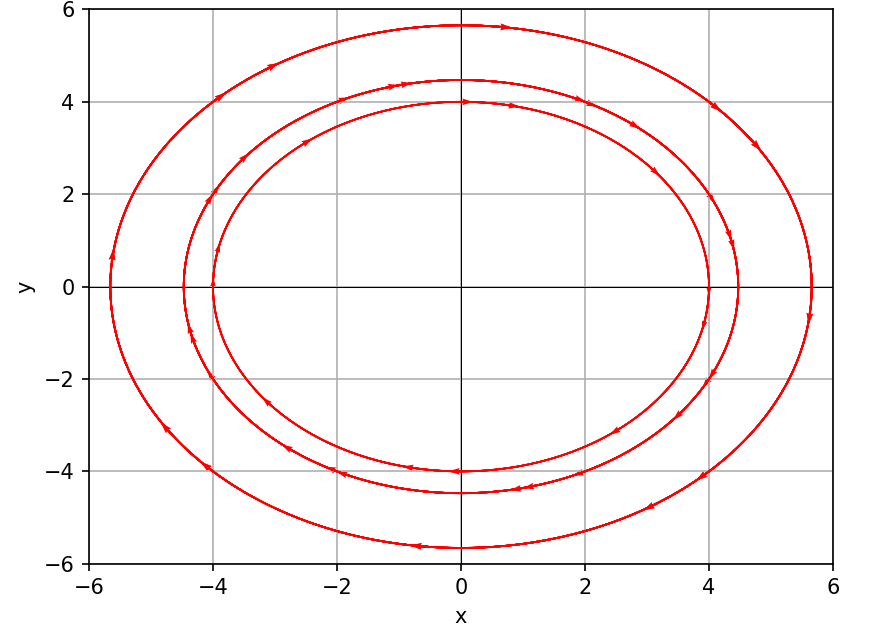
\includegraphics[width=0.4\textwidth]{img/3.png}
        \caption{(3)的相图}
    \end{figure}

    \item
    
    解$
    \begin{cases}
        2x + 3y = 0 \\
        x + 3y = 0
    \end{cases}
    $
    得平衡点为$P(0, 0)$.

    系数矩阵 $A = \begin{bmatrix} 2 & 3 \\ 1 & 3 \end{bmatrix}$,
    特征方程为 $|A - \lambda I| = 0$, 即

    $$
    \begin{vmatrix}
        2 - \lambda & 3 \\
        1 & 3 - \lambda
    \end{vmatrix} = \lambda^2 - 5\lambda + 3 = 0
    $$

    解得特征值 $\lambda_1 = \frac{5 - \sqrt{13}}{2}, \lambda_2 = \frac{5 + \sqrt{13}}{2}\quad (p=-5, q=3)$.

    这是一个不稳定结点.

    其相图如下所示:

    \begin{figure}[H]
        \centering
        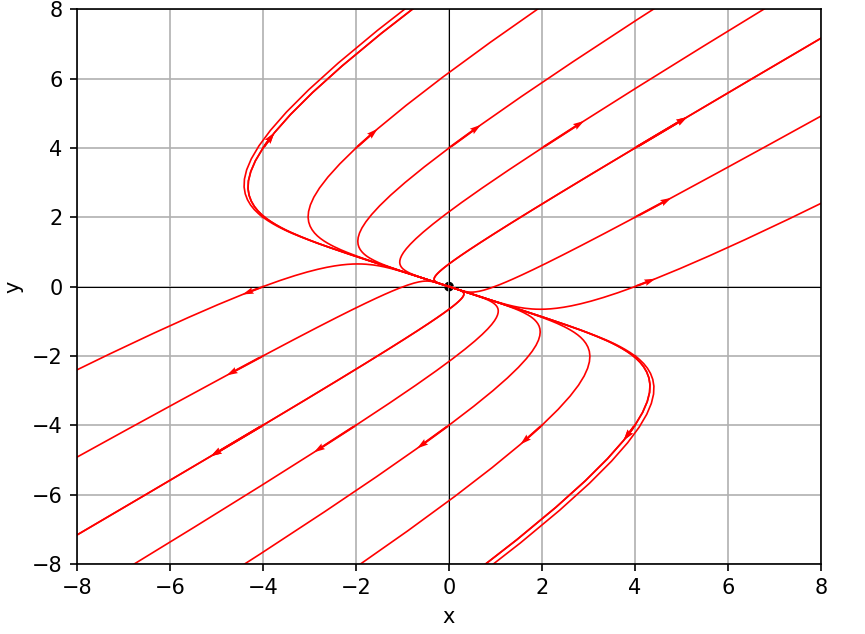
\includegraphics[width=0.4\textwidth]{img/4.png}
        \caption{(4)的相图}
    \end{figure}
\end{enumerate}

\end{document}